%% LyX 2.4.1 created this file.  For more info, see https://www.lyx.org/.
%% Do not edit unless you really know what you are doing.
\documentclass[10pt,english,t]{beamer}
\usepackage{lmodern}
\usepackage[T1]{fontenc}
\usepackage[utf8]{inputenc}
\usepackage{babel}
\usepackage{amsbsy}
\usepackage{amstext}
\usepackage{amssymb}
\usepackage{graphicx}
\usepackage[authoryear]{natbib}
\PassOptionsToPackage{normalem}{ulem}
\usepackage{ulem}
\ifx\hypersetup\undefined
  \AtBeginDocument{%
    \hypersetup{pdfusetitle,
 bookmarks=true,bookmarksnumbered=false,bookmarksopen=false,
 breaklinks=false,pdfborder={0 0 1},backref=false,colorlinks=false}
  }
\else
  \hypersetup{pdfusetitle,
 bookmarks=true,bookmarksnumbered=false,bookmarksopen=false,
 breaklinks=false,pdfborder={0 0 1},backref=false,colorlinks=false}
\fi

\makeatletter

%%%%%%%%%%%%%%%%%%%%%%%%%%%%%% LyX specific LaTeX commands.
%% Because html converters don't know tabularnewline
\providecommand{\tabularnewline}{\\}

%%%%%%%%%%%%%%%%%%%%%%%%%%%%%% Textclass specific LaTeX commands.
% this default might be overridden by plain title style
\newcommand\makebeamertitle{\frame{\maketitle}}%
% (ERT) argument for the TOC
\AtBeginDocument{%
  \let\origtableofcontents=\tableofcontents
  \def\tableofcontents{\@ifnextchar[{\origtableofcontents}{\gobbletableofcontents}}
  \def\gobbletableofcontents#1{\origtableofcontents}
}

%%%%%%%%%%%%%%%%%%%%%%%%%%%%%% User specified LaTeX commands.
\usepackage{tikz}
\usetikzlibrary{positioning}
\usepackage{appendixnumberbeamer}

\usepackage{booktabs}

\usetheme[progressbar=frametitle,block=fill]{metropolis}

% margin
\setbeamersize{text margin right=1.5cm}

% colors
\colorlet{DarkRed}{red!70!black}
\setbeamercolor{normal text}{fg=black}
\setbeamercolor{alerted text}{fg=DarkRed}
\setbeamercolor{progress bar}{fg=DarkRed}
\setbeamercolor{button}{bg=DarkRed}

% width of seperators
\makeatletter
\setlength{\metropolis@titleseparator@linewidth}{1pt}
\setlength{\metropolis@progressonsectionpage@linewidth}{1pt}
\setlength{\metropolis@progressinheadfoot@linewidth}{1pt}
\makeatother

% new alert block
\newlength\origleftmargini
\setlength\origleftmargini\leftmargini
\setbeamertemplate{itemize/enumerate body begin}{\setlength{\leftmargini}{4mm}}
\let\oldalertblock\alertblock
\let\oldendalertblock\endalertblock
\def\alertblock{\begingroup \setbeamertemplate{itemize/enumerate body begin}{\setlength{\leftmargini}{\origleftmargini}} \oldalertblock}
\def\endalertblock{\oldendalertblock \endgroup}
\setbeamertemplate{mini frame}{}
\setbeamertemplate{mini frame in current section}{}
\setbeamertemplate{mini frame in current subsection}{}
\setbeamercolor{section in head/foot}{fg=normal text.bg, bg=structure.fg}
\setbeamercolor{subsection in head/foot}{fg=normal text.bg, bg=structure.fg}

% footer
\makeatletter
\setlength{\metropolis@frametitle@padding}{1.6ex}
\setbeamertemplate{footline}{%
    \begin{beamercolorbox}[colsep=1.5pt]{upper separation line head}
    \end{beamercolorbox}
    \begin{beamercolorbox}{section in head/foot}
      \vskip1pt\insertsectionnavigationhorizontal{\paperwidth}{}{\hskip0pt plus1filll \insertframenumber{} / \inserttotalframenumber \hskip2pt}\vskip3pt% 
    \end{beamercolorbox}%
    \begin{beamercolorbox}[colsep=1.5pt]{lower separation line head}
    \end{beamercolorbox}
}
\makeatother

% toc
\setbeamertemplate{section in toc}{\hspace*{1em}\inserttocsectionnumber.~\inserttocsection\par}
\setbeamertemplate{subsection in toc}{\hspace*{2em}\inserttocsectionnumber.\inserttocsubsectionnumber.~\inserttocsubsection\par}
% Added by lyx2lyx
\setlength{\parskip}{\smallskipamount}
\setlength{\parindent}{0pt}

\AtBeginDocument{
  \def\labelitemii{-}
}

\makeatother

\begin{document}
\title{Stimulus Effects of Common Fiscal Policies}
\date{\textbf{T2M 2025}}
\author{\vspace{-4mm}\footnotesize
Tobias Broer (Paris School of Economics)\\
Jeppe Druedahl (University of Copenhagen)\\
Karl Harmenberg (University of Oslo)\\
Erik Öberg (Uppsala University)\vspace{4mm}
}

{
\setbeamertemplate{footline}{} 
\begin{frame}

\maketitle

\end{frame}
}

\addtocounter{framenumber}{-1}
\begin{frame}{Motivation}
\vspace{0.2cm}
\begin{itemize}
\item {\small\hspace{-0.2cm}}\textbf{Post-Great Recession}: Revival of
countercyclical fiscal policies

{\small\hspace{-0.2cm}}- Stimulus checks, UI increases / extensions,
firm subsidies, etc\pause \vspace{0.3cm}
\item \hspace{-0.2cm}\textbf{Vs. macro literature}: Focus on \textbf{the}
fiscal multiplier\pause  \vspace{0.3cm}
\item \hspace{-0.2cm}\textbf{This paper:} Compare stimulus from common
fiscal policies\pause \vspace{0.1cm}
\begin{enumerate}
\item Quantify absolute and relative long-run fiscal multipliers
\item Identify their main determinants
\end{enumerate}
\textbf{- HA-NK-SAM framework} to activate main policy channels
\begin{enumerate}
\item Labor-market frictions (SAM) $\Rightarrow$ cyclical hiring, firing,
unemp risk
\item Incomplete markets (HA) $\Rightarrow$ heterog. MPCs, cyclical prec
savings
\item Nominal rigidities (NK) $\Rightarrow$ demand-determined output\pause
\end{enumerate}
\textbf{- }Analytical characterisation of relative fiscal multipliers
\end{itemize}
\end{frame}
%
\begin{frame}{What we find}

\vspace{0.5cm} \hspace{-0.25cm}\textbf{1. Large range of LR fiscal
multipliers across policies (0.3-1.6)}

{\small - Retention subsidies most, stimulus checks least stimulative}\textbf{\vspace{0.25cm}}

\pause \hspace{-0.25cm}\textbf{2. Relative multipliers w.r.t. to
$\boldsymbol{G}$: }hinge on specific frictions

- \textbf{Household transfers}: Degree of partial insurance

- \textbf{Subsidies}:{\footnotesize{} Hiring/firing elasticity to LRP,
MPC o/o profits, nominal frictions}\vspace{0.25cm}

\end{frame}
%
\begin{frame}{Literature}

{\scriptsize\vspace{-1mm}}{\footnotesize\textbf{HANK-SAM:}}{\footnotesize{}
Gornemann et al. (2016), Den Haan et. al. (2018), Challe (2020), McKay-Reis
(2020), Ravn-Sterk (2021), Bilbiie (2021), Cho (2022), Graves (2022),
Kekre (2022), Gehrke et al (2023)}{\footnotesize\par}

{\scriptsize\vspace{-1mm}}{\scriptsize\textbf{HANK (fiscal policy):}}{\scriptsize{}
Kaplan et. al. (2018), Hagedorn et. al. (2019), Alves et. al. (2020),
Auclert (2023)}{\scriptsize\par}

{\scriptsize\vspace{-1mm}}{\scriptsize\textbf{SAM (inelastic entry):}}{\scriptsize{}
Coles-Kelishomi (2018), Fujita-Ramey (2007), Haefke-Reiter (2020),
Leduc-Liu (2020), Mercan et. al. (2021), Engbom (2021)}{\scriptsize\par}

{\scriptsize\vspace{-1mm}}{\scriptsize\textbf{SAM (endogenous separations):
}}{\scriptsize Mortesen-Pissarides (1994), Den Haan et. al. (2000),
Shimer (2012), Fujita-Ramey (2012), Barnichon (2012), Trigari (2019)}{\scriptsize\par}

{\scriptsize\vspace{-1mm}}{\scriptsize\textbf{RANK-SAM:}}{\scriptsize{}
Walsh (2005), Gertler et. al. (2008), Trigari (2009), Gali (2010),
Ravenna-Walsh (2012), Christiano et al. (2016)}{\scriptsize\par}

{\scriptsize\vspace{-1mm}}{\scriptsize\textbf{Consumption effects
of unemployment (risk): }}{\scriptsize Gruber (1997), Aguiar-Hurst
(2005), Eusepi-Preston (2015), Chodorow-Reich-Karabarbounis (2016),
Kolsrud et. al. (2018), Harmenberg-Öberg (2021), Graves (2022), Ganong-Noel
(2019), Ganong et. al. (2022)}{\scriptsize\par}

{\scriptsize\textbf{\vspace{-5mm}Decomposition of fiscal policies
into PE / GE: }}{\scriptsize Wolf (2023)}{\scriptsize\par}

\vspace{0.6cm}\textbf{This paper}{\small :}\vspace{-0.2cm}
\begin{itemize}
\item {\small Quantitative framework comparing several fiscal policies}{\small\par}
\item {\small Data-consistent hiring-and-firing dynamics \& partial insurance}{\small\par}
\item {\small Analytical characterisation of transmission \& of relative
fiscal multipliers}{\small\par}
\end{itemize}
\end{frame}
%


\section{Model}
\begin{frame}{Model overview}
\begin{itemize}
\item <1->\textbf{Households:}
\begin{itemize}
\item Employed: earn real wage $w$
\item Unemployed: search, earn UI (rep r $\textcolor{blue}{\overline{\phi_{t}}}$
for $\textcolor{blue}{\overline{u_{t}}}$ months, then {\footnotesize$\underline{\phi}<\textcolor{blue}{\overline{\phi_{t}}}$})
\item Consume, save in real bond; hand-to-mouth-share $\Theta$
\item Pay labor income tax, receive dividends and >>universal<< transfer
$\textcolor{blue}{T}$
\end{itemize}
\end{itemize}
\end{frame}
%
\begin{frame}{Model overview}
\begin{itemize}
\item \textbf{Households:}
\begin{itemize}
\item Employed: earn real wage $w$ 
\item Unemployed: search, earn UI (rep rate $\textcolor{blue}{\overline{\phi_{t}}}$
for $\textcolor{blue}{\overline{u_{t}}}$ months, then $\underline{\phi}$)
\item Consume, save in real bond; hand-to-mouth-share $\Theta$
\item Pay labor income tax, receive dividends and >>universal<< transfer
$\textcolor{blue}{T}$
\end{itemize}
\item \textbf{Producers:}
\begin{enumerate}
\item \textbf{Intermediate-goods producers: }Labor $\Rightarrow$ intermediate
goods
\begin{itemize}
\item Idle / open vacancy / matched with worker (profits $P_{t}^{x}-w$)
\item Heterogeneous entry costs: Sluggish vacancy creation
\item ... and continuation costs: Time-varying separations
\item >>Retention<< ($\textcolor{blue}{\underline{rs_{t}}}$) / >>hiring<<($\textcolor{blue}{\underline{hs_{t}}}$)
subsidies to all / new matches
\end{itemize}
\item \textbf{Wholesale producers: }Intermediate goods $\Rightarrow$ differentiated
goods
\begin{itemize}
\item Monopolistic competition + Rotemberg price adjustment costs
\end{itemize}
\item \textbf{Final producers: }Differentiated goods $\Rightarrow$ final
good
\end{enumerate}
\end{itemize}
\end{frame}
%
\begin{frame}{Model overview {\tiny\textbf{Details on slide }}{\tiny\ref{slide:model_details}}}
\vspace{-0.25cm}
\begin{itemize}
\item \textbf{Households:}
\begin{itemize}
\item Employed: earn real wage $w$
\item Unemployed: search, earn UI (rep rate $\textcolor{blue}{\overline{\phi_{t}}}$
for $\textcolor{blue}{\overline{u_{t}}}$ months, then $\underline{\phi}<\overline{\phi_{t}}$)
\item Consume and save in real bond; hand-to-mouth-share $\Theta$
\item Pay labor income tax, receive dividends and >>universal<< transfer
$\textcolor{blue}{T}$
\end{itemize}
\item \textbf{Producers:}
\begin{enumerate}
\item \textbf{Intermediate-good producers: }Labor $\Rightarrow$ intermediate
goods
\begin{itemize}
\item Idle; open vacancy; or matched with worker: profits $P_{x}Z-w$
\item Heterogeneous entry costs: Sluggish vacancy creation
\item ... and continuation costs: Time-varying separations
\item >>Retention<< ($\textcolor{blue}{\underline{rs_{t}}}$) / >>hiring<<($\textcolor{blue}{\underline{hs_{t}}}$)
subsidies to all / new matches
\end{itemize}
\item \textbf{Wholesale producers: }Intermediate goods $\Rightarrow$ differentiated
goods
\begin{itemize}
\item Monopolistic competition + Rotemberg price adjustment costs
\end{itemize}
\item \textbf{Final producers: }Differentiated goods $\Rightarrow$ final
good
\end{enumerate}
\item \textbf{Government:}
\begin{enumerate}
\item (Long-term) debt smoothes labor-income taxes
\item Policies: $\textcolor{blue}{G}_{t}$, $\textcolor{blue}{T}_{t}$,
$\textcolor{blue}{\overline{\phi_{t}}}$, $\textcolor{blue}{\overline{u_{t}}}$,
$\textcolor{blue}{rs_{t}}$, $\textcolor{blue}{hs_{t}}$
\end{enumerate}
\item \textbf{Central bank}: Nominal interest rate follows Taylor rule
\end{itemize}
\end{frame}
%
\begin{frame}{Model analysis in sequence space}
\textbf{\label{slide:analytics}\vspace{0.25cm}}
\begin{itemize}
\item >>MIT<< perturbation $\boldsymbol{\epsilon}$ to policy paths

\hspace{0.25cm}- E.g. ${\bf {g}}=[g_{0},g_{1},g_{2},...]$\textbf{\vspace{0.3cm}}
\item \textbf{Aim}: Study transition of endog variables back to steady state
\textbf{\vspace{0.3cm}}
\item \textbf{Problem}: Complex model, many variables\textbf{\vspace{0.3cm}}
\item \textbf{Insights}: 
\begin{enumerate}
\item Can group variables in >>blocks<< with few inputs / outputs
\begin{itemize}
\item Simplifies computation
\end{itemize}
\item Circular input-output relation among HA-NK-SAM blocks
\item Circles break transmission into direct effects and GE feedback
\end{enumerate}
\end{itemize}
\end{frame}
%

\section{Analytical Characterisation}
\begin{frame}{Equilibium transmission as a >>directed cycle graph<<}

\hspace{0.5cm} \vspace{1cm}

\includegraphics[bb=0bp 0bp 656bp 190bp,clip,width=1.13\linewidth]{figs/model_diagram}\vspace{1cm}

\end{frame}
%
\begin{frame}{Directed cycle graph-representation: Implications}

\hspace{7cm} \vspace{-0.3cm}

\includegraphics[bb=0bp 0bp 656bp 190bp,clip,width=0.85\linewidth]{figs/model_diagram}\vspace{-0.1cm}
\begin{itemize}
\item \textbf{Policies}: work through >>their<< blocks' outputs 

\hspace{-0.25cm}- e.g. HH transfers, G: through $\boldsymbol{r}$
via asset demand/supply (HA)\pause
\item Allows\textbf{ Decomposition of policy effects}:
\end{itemize}
\hspace{1cm} \uline{Policy-specific} direct effect $\times$ \uline{common
}GE multiplier\pause
\begin{itemize}
\item \textbf{Policy comparison} hinges on direct effects only {\tiny\textbf{To
}}{\tiny Propositions \ref{slide:Prop1}}\pause \vspace{0.5cm}
\item \textbf{Now}: Quantitative analysis
\end{itemize}
\end{frame}
%

\section{Calibration\protect\label{sec:calib}}
\begin{frame}{Our calibration approach}
\label{slide:calib}
\begin{itemize}
\item \textbf{Key to fiscal transmission:}
\begin{enumerate}
\item Transfers: HH consumption insurance (MPC, prec. savings)
\item Subsidies: Hiring/ firing response to movements in LRP \pause
\end{enumerate}
\end{itemize}
\begin{enumerate}
\item \textbf{$\Rightarrow$ HA block:} Given UI (Kekre 23), choose $B,\beta_{i},\Theta$
to match
\begin{itemize}
\item SS real interest rate $(2$ percent)
\item Cons. of unemployed vs. employed (Chodorow-Reich et al 2016)
\item Cons. response to UI-benefit expiration (Ganong et al 19)
\item MPC not targeted but in line with data\vspace{0.3cm}\pause
\end{itemize}
\item \textbf{$\Rightarrow$ SAM block:}{\small{} }{\footnotesize Choose $W,$
shape of separation/entry costs $\psi/\xi$ to match}{\footnotesize\par}
\begin{itemize}
\item $u_{t}$-response to aggregate productivity shocks in U.S. 
\item Lead-lag separation vs job-finding (Broer et al 2023)
\item ... and their contributions to $u_{t}$ dynamics (Broer et al 2023)\pause
\end{itemize}
\end{enumerate}
\begin{itemize}
\item \textbf{Rest}: standard values / macro targets{\tiny\textbf{ Details
on slide }}{\tiny\ref{sec:calib_detail}}{\tiny\textbf{ Parameter
tables on slide }}{\tiny\ref{slide:calib_detail1}}{\tiny\textbf{ }}{\tiny\par}
\end{itemize}
\end{frame}
%

\section{Quantitative Analysis \protect\label{sec:Quantitative-Analysis}}

\begin{frame}{Quantitative Analysis}
\label{slide:Quant}

\vspace{2cm}\centering
\begin{enumerate}
\item Quantify absolute \& relative fiscal multipliers in baseline model
\item Quantify their determinants by varying individual frictions
\end{enumerate}
\end{frame}
%
\begin{frame}{Baseline calibration: Policy paths and fiscal costs}

\centering%
\begin{tabular}{ccc}
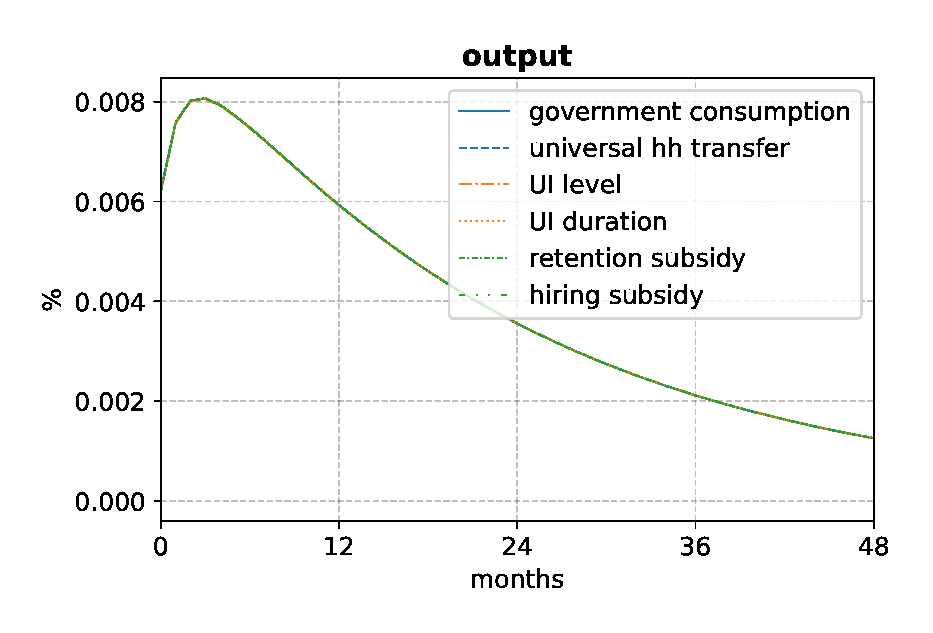
\includegraphics[width=0.52\linewidth]{results/policies_Y_titled} &  & 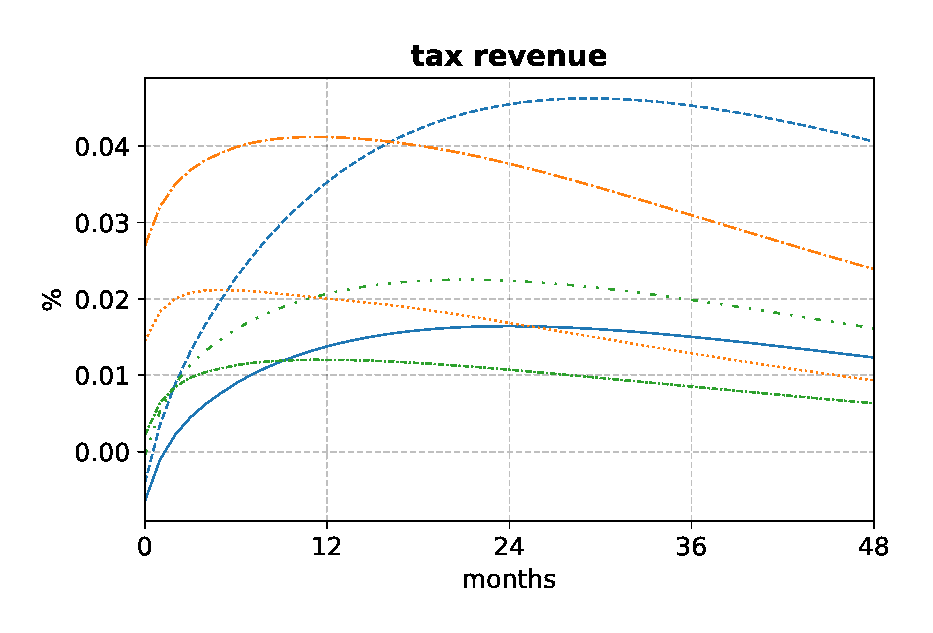
\includegraphics[width=0.52\linewidth]{results/policies_tax_titled}\tabularnewline
\end{tabular}
\begin{itemize}
\item Baseline policy: Persistent \textbf{G} shock ($\rho_{G}=0.965$).
\item Other policies chosen to yield identical output paths
\item Yet, starkly different paths of tax revenues
\end{itemize}
\end{frame}
%
\begin{frame}{Baseline calibration: Fiscal multipliers relative to \textbf{G}}

\begin{table}
\begin{center}
\begin{tabular}{lcccccc}
\toprule
& &  \multicolumn{3}{c}{\hrulefill\,\,\textbf{HH transfers}\,\,\hrulefill} & \multicolumn{2}{c}{\hrulefill\,\,\textbf{Firm subsidies}\,\,\hrulefill} \\
& \textbf{G} [level] & \textbf{Transfer} & \textbf{Level} & \textbf{Duration} & \textbf{Retain} & \textbf{Hire} \\
\midrule
& 1.0 [0.99] & 0.28 & 0.44 & 1.03 & 1.64 & 0.72 \\
\bottomrule
\end{tabular}
  
\end{center}
\vspace{-2mm}
\end{table}
\vspace{1cm}
\begin{itemize}
\item Strong dispersion in fiscal costs and multipliers.
\item Retention subsidies most, universal transfers least stimulative
\end{itemize}
\end{frame}

\begin{frame}{Determinants of fiscal multipliers}
\vspace{1cm}
\begin{itemize}
\item Identify determinants by reducing frictions one-by-one
\end{itemize}
\end{frame}
%
\begin{frame}{Determinants of fiscal multipliers}

\centering
\begin{small}
\setlength\tabcolsep{1.5pt} 
\begin{tabular}{lcccccc}
\toprule
& &  \multicolumn{3}{c}{\hrulefill\,\,\textbf{Household transfers}\,\,\hrulefill} & \multicolumn{2}{c}{\hrulefill\,\,\textbf{Firm transfers}\,\,\hrulefill} \\
& \textbf{G} [level] & \textbf{Transfer} & \textbf{Level} & \textbf{Duration} & \textbf{Retain} & \textbf{Hire} \\
\midrule
1. Baseline & 1.0 [0.99] & 0.28 & 0.44 & 1.03 & 1.64 & 0.72 \\
\midrule
2. Less sticky $P$ ($\phi \!=\! 178$) &&&&&&\\
3. Reactive mp ($\delta_\pi \!=\! 2$)  &&&&&&\\
\midrule
4. Representative agent &&&&&& \\
5. Fewer HtM (17.4\%)   &&&&&&\\
6. Reactive tax ($\omega \!=\! 0.10$) &&&&&& \\
\midrule
7. Ex. separations ($\psi \!=\! 0$)  &&&&&&\\
8. Free entry ($\xi \!=\! \infty$)  &&&&&& \\
9. Wage rule ($\eta_e \!=\! 0.50$)   &&&&&&\\
10. 95\% of div. to PIH   &&&&&&\\
\bottomrule
\end{tabular}
  
\end{small}
\vspace{-2mm}
\end{frame}
%
\begin{frame}{Benchmark $\boldsymbol{G}$ multiplier}

\centering
\begin{small}
\setlength\tabcolsep{1.5pt} 
\input{results/fiscal_multipliers_all_pres_G_1.tex}  
\end{small}
\vspace{-2mm}
\begin{itemize}
\item Government-consumption multipliers increase with ...
\begin{itemize}
\item Nominal rigidity, passive MP, debt-financing, less-Ricardian HHs (Auclert
et al 2024, Hagedorn et al 2023) 
\end{itemize}
\end{itemize}
\end{frame}
%
\begin{frame}{Benchmark $\boldsymbol{G}$ multiplier}

\centering
\begin{small}
\setlength\tabcolsep{2.5pt} 
\begin{tabular}{lcccccc}
\toprule
& &  \multicolumn{3}{c}{\hrulefill\,\,\textbf{Household transfers}\,\,\hrulefill} & \multicolumn{2}{c}{\hrulefill\,\,\textbf{Firm transfers}\,\,\hrulefill} \\
& \textbf{G} [level] & \textbf{Transfer} & \textbf{Level} & \textbf{Duration} & \textbf{Retain} & \textbf{Hire} \\
\midrule
1. Baseline & 1.0 [\color{red}{\textbf{0.99}}] & 0.28 & 0.44 & 1.03 & 1.64 & 0.72 \\
\midrule
2. Less sticky $P$ ($\phi \!=\! 178$) & 1.0 [\color{red}{\textbf{0.61}}] &&&&& \\
3. Reactive mp ($\delta_\pi \!=\! 2$) & 1.0 [\color{red}{\textbf{0.64}}]  &&&&&\\
\midrule
4. Representative agent & 1.0 [\color{red}{\textbf{0.54}}] &&&&& \\
5. Fewer HtM (17.4\%) & 1.0 [\color{red}{\textbf{0.80}}] &&&&& \\
6. Reactive tax ($\omega \!=\! 0.10$) & 1.0 [\color{red}{\textbf{0.84}}]&&&&&  \\
\midrule
7. Ex. separations ($\psi \!=\! 0$) & 1.0 [\color{red}{\textbf{0.13}}] &&&&& \\
8. Free entry ($\xi \!=\! \infty$) & 1.0 [\color{red}{\textbf{0.54}}]  &&&&&\\
9. Wage rule ($\eta_e \!=\! 0.50$) & 1.0 [\color{red}{\textbf{0.73}}]  &&&&&\\
10. 95\% of div. to PIH & 1.0 [\color{red}{\textbf{0.82}}] &&&&& \\
\bottomrule
\end{tabular}
  
\end{small}
\vspace{-2mm}
\begin{itemize}
\item Government-consumption multiplier increases with ...
\begin{itemize}
\item Nominal rigidity, passive MP, debt-financing, less-Ricardian HHs
\item SAM frictions, wage rigidity, MPC o/o profits
\end{itemize}
\end{itemize}
\end{frame}
%
\begin{frame}{Relative HH-transfer multipliers: non-HA frictions}

\centering
\begin{small}
\setlength\tabcolsep{2.5pt} 
\begin{tabular}{lcccccc}
\toprule
& &  \multicolumn{3}{c}{\hrulefill\,\,\textbf{Household transfers}\,\,\hrulefill} & \multicolumn{2}{c}{\hrulefill\,\,\textbf{Firm transfers}\,\,\hrulefill} \\
& \textbf{G} [level] & \textbf{Transfer} & \textbf{Level} & \textbf{Duration} & \textbf{Retain} & \textbf{Hire} \\
\midrule
1. Baseline & 1.0 [0.99] &  \color{red}{\textbf{0.28}} &  \color{red}{\textbf{0.44}} &  \color{red}{\textbf{1.03}} & & \\
\midrule
2. Less sticky $P$ ($\phi \!=\! 178$) & 1.0 [0.61] & \color{red}{\textbf{0.30}} & \color{red}{\textbf{0.47}} & \color{red}{\textbf{1.03}} & & \\
3. Reactive mp ($\delta_\pi \!=\! 2$) & 1.0 [0.64] & \color{red}{\textbf{0.30}} & \color{red}{\textbf{0.47}} & \color{red}{\textbf{1.03}} & & \\
\midrule
4. Representative agent & 1.0 [0.54] & 0.00 & 0.00 & 0.00 && \\
5. Fewer HtM (17.4\%) & 1.0 [0.80] & 0.19 & 0.41 & 1.11 & & \\
6. Reactive tax ($\omega \!=\! 0.10$) & 1.0 [0.84] & 0.19 & 0.40 & 1.10 & & \\
\midrule
7. Ex. separations ($\psi \!=\! 0$) & 1.0 [0.13] & \color{red}{\textbf{0.35}} & \color{red}{\textbf{0.52}} & \color{red}{\textbf{1.02}} & & \\
8. Free entry ($\xi \!=\! \infty$) & 1.0 [0.54] & \color{red}{\textbf{0.31}} & \color{red}{\textbf{0.47}} & \color{red}{\textbf{1.03}} & &\\
9. Wage rule ($\eta_e \!=\! 0.50$) & 1.0 [0.73] & \color{red}{\textbf{0.29}} & \color{red}{\textbf{0.46}} & \color{red}{\textbf{1.03}} & & \\
10. 95\% of div. to PIH & 1.0 [0.82] & \color{red}{\textbf{0.28}} & \color{red}{\textbf{0.43}} & \color{red}{\textbf{0.99}} & & \\
\bottomrule
\end{tabular}
  
\end{small}
\vspace{-2mm}
\begin{itemize}
\item Relative HH transfer multipliers $\approx$ unaffected by non-HA frictions
\end{itemize}
\end{frame}
%
\begin{frame}{Relative HH-transfer multipliers: HA frictions}

\centering
\begin{small}
\setlength\tabcolsep{2.5pt} 
\begin{tabular}{lcccccc}
\toprule
& &  \multicolumn{3}{c}{\hrulefill\,\,\textbf{Household transfers}\,\,\hrulefill} & \multicolumn{2}{c}{\hrulefill\,\,\textbf{Firm transfers}\,\,\hrulefill} \\
& \textbf{G} [level] & \textbf{Transfer} & \textbf{Level} & \textbf{Duration} & \textbf{Retain} & \textbf{Hire} \\
\midrule
1. Baseline & 1.0 [0.99] & 0.28 & 0.44 & 1.03 & 1.64 & 0.72 \\
\midrule
2. Less sticky $P$ ($\phi \!=\! 178$) & 1.0 [0.61] & 0.30 & 0.47 & 1.03 & & \\
3. Reactive mp ($\delta_\pi \!=\! 2$) & 1.0 [0.64] & 0.30 & 0.47 & 1.03 & &\\
\midrule
4. Representative agent & 1.0 [0.54] & \color{red}{\textbf{0.00}} & \color{red}{\textbf{0.00}} & \color{red}{\textbf{0.00}} && \\
5. Fewer HtM (17.4\%) & 1.0 [0.80] & \color{red}{\textbf{0.19}} & \color{red}{\textbf{0.41}} & \color{red}{\textbf{1.11}} & 1& \\
6. Reactive tax ($\omega \!=\! 0.10$) & 1.0 [0.84] & \color{red}{\textbf{0.19}} & \color{red}{\textbf{0.40}} & \color{red}{\textbf{1.10}} & & \\
\midrule
7. Ex. separations ($\psi \!=\! 0$) & 1.0 [0.13] & 0.35 & 0.52 & 1.02 && \\
8. Free entry ($\xi \!=\! \infty$) & 1.0 [0.54] & 0.31 & 0.47 & 1.03 && \\
9. Wage rule ($\eta_e \!=\! 0.50$) & 1.0 [0.73] & 0.29 & 0.46 & 1.03 & & \\
10. 95\% of div. to PIH & 1.0 [0.82] & 0.28 & 0.43 & 0.99 & & \\
\bottomrule
\end{tabular}
  
\end{small}
\vspace{-2mm}
\begin{itemize}
\item Ricardian households: zero transfer multipliers
\item Lower MPC lowers transfer multipliers \& \uline{raises} duration multiplier
\item Same holds for more tax financing
\end{itemize}
\end{frame}
%
\begin{frame}{Relative firm-subsidy multipliers: non-SAM frictions}

\centering
\begin{small}
\setlength\tabcolsep{2.5pt} 
\input{results/fiscal_multipliers_all_pres_S.tex}  
\end{small}
\vspace{-2mm}
\begin{itemize}
\item Relative multipliers of subsidies $\approx$ unaffected by non-SAM
frictions
\item Less nominal rigidity: subsidies more effective wrt HH transfers/$G$
\end{itemize}
\end{frame}
%
\begin{frame}{Relative firm-subsidy multipliers: SAM frictions}

\centering
\begin{small}
\setlength\tabcolsep{2.5pt} 
\input{results/fiscal_multipliers_all_pres_S_SAM.tex}  
\end{small}
\vspace{-2mm}
\begin{itemize}
\item {\small Hiring subsidy more effective with higher entry/lower separation
elasticity}{\small\par}
\item Lower MPC o/o profits weakens both subsidies
\end{itemize}
\end{frame}

\section{Extensions and robustness\protect 
%
}
%
\begin{frame}{Robustness - policy persistence}

\vspace{-6mm}
\begin{center}\begin{table}
\footnotesize
\begin{tabular}{lcccccc}
\toprule
& & & \multicolumn{2}{c}{\hrulefill\,\,\textbf{UI}\,\,\hrulefill} & \multicolumn{2}{c}{\hrulefill\,\,\textbf{Subsidies}\,\,\hrulefill} \\
& \textbf{G} [level] & \textbf{Transfer} & \textbf{Level} & \textbf{Duration} & \textbf{Retention} & \textbf{Hiring} \\
\midrule
Baseline, $\rho_G^{\frac{1}{3}} = 0.90$ & 1.0 [0.99] & 0.28 & 0.44 & 1.03 & 1.64 & 0.72 \\
$\rho_G^{\frac{1}{3}} = 0.85$ & 1.0 [1.38] & 0.22 & 0.33 & 0.71 & 0.83 & 0.50 \\
$\rho_G^{\frac{1}{3}} = 0.80$ & 1.0 [1.68] & 0.19 & 0.27 & 0.54 & 0.55 & 0.39 \\
\bottomrule
\end{tabular}

\end{table}\end{center}
\vspace{-4mm}
\begin{itemize}
\item Transfer-, subsidy multipliers boosted by higher persistence
\end{itemize}
\end{frame}
%
\begin{frame}{Extensions}
\vspace{0.5cm}
\begin{itemize}
\item Additional analysis
\begin{itemize}
\item Alternative policy paths ($\checkmark)$
\item State dependence (Future research)
\end{itemize}
\item Additional model elements
\begin{itemize}
\item Endogenous search ($\checkmark)$
\item Limited information, behavioral elements, capital (Future research)
\end{itemize}
\end{itemize}
\end{frame}
%

\section{Conclusion}
\begin{frame}{Concluding thoughts}
\vspace{0.5cm}
\begin{itemize}
\item Analysis inspired by Great Recession / COVID
\begin{itemize}
\item Temporary fiscal expansions
\item Metric: Policy effect on (cumulative) output/employment
\item Short-run demand and supply focus
\item No uncertainty, debt sustainable by assumption\pause
\end{itemize}
\item Vs. Today: Fiscal >>adjustment<<, sectoral expansions
\begin{itemize}
\item Permanent reductions in primary deficit, debt/GDP
\item Permanently higher defence spending\pause
\end{itemize}
\item Framework allows analysis of profit rates, labor re-allocation, ...\pause
\item ... but needs extensions 
\begin{itemize}
\item Permanent tax increases / exp reductions
\item Long-run supply effects
\item Multiple sectors, more fiscal structure
\item Expectations and uncertainty (entitlements, taxes, default) crucial
\end{itemize}
\end{itemize}
\end{frame}
%
\begin{frame}

\maketitle

\end{frame}
\begin{frame}{Extra slides}
\end{frame}
%
\begin{frame}{Model details}
\label{slide:model_details}
\end{frame}
%
\begin{frame}{Model details: Savers' problem and income process}
\vspace{-3mm}

{\footnotesize
\begin{align*}
V_{t}^{w}(\beta_{i},u_{it},\text{UI}_{it},a_{it-1})= & \max_{c_{it},a_{it}}\frac{c_{it}^{1-\sigma}}{1-\sigma}+\beta_{i}\mathbb{E}_{t}\left[V_{t+1}^{w}\left(\beta_{i},u_{it+1},\text{UI}_{it+1},a_{it}\right)\right]\\
\text{s.t. } & a_{it}+c_{it}=R_{t}^{\text{real}}a_{it-1}+\text{T}_{t}+\text{dividends}_{t}+(1-\tau_{t})y_{t}(u_{it},U_{it})\\
 & a_{it}\geq0
\end{align*}
for $u_{it}$ }{\footnotesize\emph{unemployment duration, $\text{UI}_{it}$
UI-eligibility, $T_{t}$}}{\footnotesize{} lump-sum transfer}{\footnotesize\emph{.}}{\footnotesize\par}
\begin{itemize}
\item \textbf{Income process} with data-consistent UI system:
\begin{enumerate}
\item \textbf{Separation rate} for employed: $\delta_{t}$
\item \textbf{Job-finding rate }for unemployed: $\lambda_{t}^{u,s}s(u_{it})$

{\footnotesize (where $s(u_{it})$ is exogenous search effectiveness)}{\footnotesize\par}
\item \textbf{Real wage}: $w_{t}$
\item \textbf{Labor-income tax: }$\tau_{t}$
\item Duration-dependent \textbf{UI system:}\vspace{1mm}

{\footnotesize a) High placement rate}{\footnotesize\textbf{ $\overline{\phi}_{t}$,
}}{\footnotesize first $\overline{u}_{t}$ months}{\footnotesize\par}

{\footnotesize b) Low replacement rate }{\footnotesize\textbf{$\underline{\phi}$,}}{\footnotesize{}
after $\overline{u}_{t}$ months}{\footnotesize\par}

{\footnotesize c) With probability $1-\pi^{UI}$, households receive
low UI immediately}{\footnotesize\par}
\end{enumerate}
\item \textbf{Policy variables}: $T_{t}$,{\footnotesize\textbf{ $\overline{\phi}_{t}$,}}{\footnotesize{}
$\overline{u}_{t}$}{\footnotesize\par}
\item \textbf{Extension:} endogenous search effort
\end{itemize}
\end{frame}
%
\begin{frame}{Model details: Search-and-matching I}
\begin{itemize}
\item \textbf{Job value }and \textbf{separation rate}, $\delta_{t}$, with
elasticity $\psi$ {\small
\begin{align*}
V_{t}^{j} & =p_{t}^{x}Z_{t}-(w_{t}-\text{rs}_{t})+\beta^{\text{firm}}\mathbb{E}_{t}\left[(1-\delta_{t+1})(V_{t+1}^{j}-\mu_{t+1}^{j})\right]\\
\delta_{t} & =\delta_{ss}\left(\frac{V_{t}^{j}}{V_{ss}^{j}}\right)^{-\psi},\,\,\,\mu_{t+1}^{j}\text{ is continuation cost}
\end{align*}
}{\small\par}
\item \textbf{Vacancy value }and \textbf{entry}, $\iota_{t}$,\textbf{ }with
elasticity\textbf{ $\xi$}{\small
\begin{align*}
V_{t}^{v} & =-\kappa+\lambda_{t}^{v}(V_{t}^{j}+\text{hs}_{t})+(1-\lambda_{t}^{v})(1-\delta_{ss})\beta^{\text{firm}}\mathbb{E}_{t}\left[V_{t+1}^{v}\right]\\
\iota_{t} & =\iota_{ss}\left(\frac{V_{t}^{v}}{V_{ss}^{v}}\right)^{\xi}
\end{align*}
}{\small\par}
\item \textbf{Microfoundation:} Continuation and entry costs drawn i.i.d.
from suitably chosen power distributions (Coles-Kelishomi, 2018)
\item \textbf{Wage rule: $w_{t}=w_{ss}\left(\frac{1-u_{t}}{1-u_{ss}}\right)^{\eta_{e}}$}
\item \textbf{Policy variables}: $rs_{t}$, $hs_{t}$
\end{itemize}
\end{frame}
%
\begin{frame}{Model details: Search-and-matching II}
\begin{itemize}
\item \textbf{Vacancy dynamics:}\vspace{-2mm}\textbf{
\begin{align*}
\tilde{v}_{t} & =(1-\delta_{ss})v_{t-1}+\iota_{t}\\
v_{t} & =(1-\lambda_{t}^{v})\tilde{v}_{t}
\end{align*}
}
\item \textbf{Unemployed and effective searchers:}\vspace{-2mm}
\begin{align*}
S_{t} & =\int\varphi(u_{it})d\boldsymbol{D}_{t}\\
u_{t} & =u_{t-1}+\delta_{t}(1-u_{t-1})-\lambda_{t}^{u,s}S_{t}
\end{align*}
\item \textbf{Tightness, $\theta_{t}=\frac{\tilde{v}_{t}}{Su_{t}}$, and
matching function:}
\begin{align*}
\lambda_{t}^{v} & =A\theta_{t}^{-\alpha}\\
\lambda_{t}^{u,s} & =A\theta_{t}^{1-\alpha}\\
\lambda_{t}^{u} & =\frac{\lambda_{t}^{u,s}S_{t}}{u_{t-1}}
\end{align*}
\end{itemize}
\end{frame}
%
\begin{frame}{Model details: Government and monetary policy}
\begin{itemize}
\item \textbf{Fiscal rule:
\[
\tau_{t}=\omega\tilde{\tau}_{t}+(1-\omega)\tau_{ss}
\]
}where $\tilde{\tau}_{t}=\frac{(1+q_{t}\delta_{q})B_{t-1}+\text{expenses}_{t}-q_{ss}B_{ss}}{\tilde{Y}_{t}^{hh}}$
implies $B_{t}=B_{SS}$
\item \textbf{Government budget with long-term bonds:}{\small
\begin{align*}
q_{t}(B_{t}-\delta_{q}B_{t-1})= & B_{t-1}\\
 & +(1-\tau_{t})\left(\overline{\phi}_{t}\text{UI}_{t}^{hh}+\underline{\phi}\left(u_{t}-\text{UI}_{t}^{hh}\right)\right)w_{t}\\
 & +\text{T}_{t}+G_{_{t}}\\
 & +\text{rs}_{t}\cdot(1-u_{t})\\
 & +\text{hs}_{t}\cdot\lambda_{t}^{v}((1-\delta_{ss})v_{t-1}+\iota_{t})\\
 & -\tau_{t}(1-u_{t})w_{t}
\end{align*}
where $\text{UI}_{t}^{hh}$ is share of households on UI}{\small\par}
\item \textbf{Central bank's Taylor rule}
\begin{equation}
R_{t}=R_{ss}\Pi_{t}^{\phi_{\pi}},\label{eq:taylor}
\end{equation}
\end{itemize}
{\tiny\textbf{To model analytics}}{\tiny\ref{slide:analytics}}{\tiny\par}
\end{frame}
%
\begin{frame}{Proposition I: Equilibium transmission as a directed cycle graph}
\label{slide:Prop1}

\hspace{2cm} \vspace{-1.2cm}\includegraphics[bb=0bp 0bp 656bp 190bp,clip,width=1\linewidth]{figs/model_diagram}\vspace{1cm}

An equilibrium of our model can to a first order be written as
\begin{align}
\boldsymbol{r^{real}} & =M_{HA}\boldsymbol{inc}+M_{d,r}\boldsymbol{d}+\text{\ensuremath{M_{s,r}\boldsymbol{s}},}\label{eq:HA-1-2-1}\\
\boldsymbol{p^{x}} & =M_{NK}\boldsymbol{r^{real}},\label{eq:NK-1-2-1}\\
\boldsymbol{inc} & \boldsymbol{=}M_{SAM}\boldsymbol{p^{x}}+\text{\ensuremath{M_{s,\text{inc}}\boldsymbol{s}}},\label{eq:SAM-1-2-1}
\end{align}
and can thus be represented by a \emph{directed cycle graph.}

{\tiny\textbf{To calibration}}{\tiny{} \ref{slide:taking_stock}}{\tiny\par}

\end{frame}
%
\begin{frame}{Proposition II: Decomposition of policy effects - PE vs GE}

\begin{equation}
\boldsymbol{inc}=\underset{\text{GE}}{\underbrace{\mathcal{G}}}\times\underset{\text{first round, demand-side policy}}{\underbrace{\boldsymbol{(}M_{\text{SAM}}M_{\text{NK}}\underset{\text{direct}}{\underbrace{M_{d,r}\boldsymbol{d}}}}}+\underset{\text{first round, supply-side policy}}{\underbrace{M_{SAM}M_{NK}\underset{\text{direct}}{\underbrace{M_{s,r}\boldsymbol{s}}}+\underset{\text{direct}}{\underbrace{M_{s,\text{inc}}\boldsymbol{s\boldsymbol{)}}}}}},\label{eq:PE_GE-1-1}
\end{equation}
where
\[
\mathcal{G}=(I-M_{SAM}M_{NK}M_{HA})^{-1}.
\]

\textbf{Implies:}
\begin{enumerate}
\item {\small Unique bounded equilibrium if }{\small\par}
\begin{itemize}
\item {\small >>local block determinacy<<}{\small\par}
\item {\footnotesize$||M_{SAM}M_{NK}M_{HA}||<1$}{\footnotesize\par}
\end{itemize}
\item GE amplification decomposed into three (HA-NK-SAM) blocks
\item Direct effects sufficient for policy comparison
\item Identical $\boldsymbol{y}$: fiscal effectiveness hinges only on (direct)
fiscal costs.
\end{enumerate}
{\tiny\textbf{To calibration}}{\tiny{} \ref{slide:taking_stock}}{\tiny\par}
\end{frame}
%
\begin{frame}{Proposition III: Relative fiscal costs of demand-side policies}

Consider sequences $\boldsymbol{d}^{0}$,$\boldsymbol{d}^{1}$ with
identical PE interest-rate responses, implying identical GE output
response $\boldsymbol{y}$.

The difference in total cumulative fiscal costs in GE equals that
in PE\vspace{-0.5cm}

\begin{equation}
\Delta\boldsymbol{taxes}=\boldsymbol{1}^{\prime}\boldsymbol{taxes}^{0}-\boldsymbol{1}^{\prime}\boldsymbol{taxes}^{1}=\boldsymbol{1}^{\prime}M_{d,\text{taxes}}\boldsymbol{d}^{0}-\boldsymbol{1}^{\prime}M_{d,\text{taxes}}\boldsymbol{d}^{1}\label{eq:proIIb-1-1}
\end{equation}

So $\Delta\boldsymbol{taxes}$ unaffected by changes in the model
outside the \emph{HA }block.\pause\vspace{0.5cm}

\textbf{Intuition}: 

{\footnotesize Common GE transmission \& PE int. rate $\Rightarrow$
common GE expenditure, cancels in (\ref{eq:proIIb-1-1})}\pause

\textbf{Implication}: 

{\small\uline{Relative}}{\small{} stimulus of HH transfers}{\small\textbf{
/$G$ }}{\small unaffected by NK \& SAM frictions}\pause

\textbf{Firm Subsidies:}

Holds in the limit of complete markets {\tiny\textbf{To calibration}}{\tiny{}
\ref{slide:taking_stock}}{\tiny\par}
\end{frame}
%
\begin{frame}{From fiscal costs to multipliers}
\begin{itemize}
\item Most common policy Metric: cumulative Fiscal Multiplier
\end{itemize}
\[
\mathcal{M}=\text{cumulative fiscal multiplier}=\frac{\boldsymbol{1}^{\prime}\boldsymbol{y}}{\boldsymbol{1}^{\prime}\boldsymbol{taxes}}.
\]

\begin{itemize}
\item Identical $\boldsymbol{y}$ response:
\end{itemize}
\hspace{1cm} Ratio of FMs = ratio of \textbf{total} net spending/taxes
\begin{itemize}
\item \textbf{Demand-side policies}: Relative FMs after change in non-HA
parameters 
\begin{align*}
\frac{\mathcal{M}_{d^{1}}^{\text{new}}}{\mathcal{M}_{d^{0}}^{\text{new}}} & =\frac{\boldsymbol{1}^{\prime}\boldsymbol{taxes}_{0}^{\text{new}}}{\boldsymbol{1}^{\prime}\boldsymbol{taxes}_{1}^{\text{new}}}=\frac{\boldsymbol{1}^{\prime}M_{d,\text{taxes}}\boldsymbol{d}^{0}+\boldsymbol{1}^{\prime}\boldsymbol{taxes}_{}^{\text{GE}}}{\boldsymbol{1}^{\prime}M_{d,\text{taxes}}\boldsymbol{d}^{1}+\boldsymbol{1}^{\prime}\boldsymbol{taxes}_{}^{\text{GE}}}
\end{align*}
\item \textbf{Relative FMs unaffected by parameter changes if }
\begin{itemize}
\item ... change in GE tax revenue small to original total revenue
\item ... or if original FMs similar {\tiny\textbf{To calibration}}{\tiny{}
\ref{slide:taking_stock}}{\tiny\par}
\end{itemize}
\end{itemize}
\end{frame}
%
\begin{frame}{Unemployment risk \& consumption insurance: 4 calibration targets}
\label{sec:calib_detail}

\begin{itemize}
\item \textbf{Stylized fact \#1: }Consumption \textasciitilde 20\% lower
for unemployed (Chodorow-Reich-Karabarbounis, 2016)
\item \textbf{Stylized fact \#2: }Drop at UI exhaustion of \textasciitilde 45\%
of income drop (Ganong-Noel, 2019)
\item \textbf{Stylized Fact \#3:}\emph{ Separation rate leads job-finding
rate by 9-16 months}\vspace{3mm}
\begin{itemize}
\item In response to technology and monetary shocks (Broer et al 2023)
\item ... and \emph{uncertainty shocks} (Oh-Picco, 2020).
\end{itemize}
\item \textbf{Stylized Fact \#4:}\emph{ Separations account for 40-60\%
of unemployment }variation \vspace{3mm}
\begin{itemize}
\item In response to technology and monetary shocks (Broer et al 2023)
\item ... \emph{uncertainty shocks} (Oh-Picco, 2020)
\item ... and unconditionally.
\end{itemize}
\end{itemize}
\end{frame}
%
\begin{frame}{Unemployment and consumption}
\label{sec:calib_detail-1}

\begin{center}
\includegraphics[width=0.7\linewidth]{../Freie_Univ_Berlin_may_2023/figs/Ganong19}
\par\end{center}

\begin{center}
\vspace{-3mm}{\footnotesize\textbf{Source:}}{\footnotesize{} Ganong-Noel
(2019)}{\footnotesize\par}
\par\end{center}

\end{frame}
%
\begin{frame}{Unemployment and consumption}
\begin{itemize}
\item Targets: Annual IR 2 \%, cons drop in unemployment, and at expiration
\item Model parameters: bond supply $B,$share of HTM, discount factor $\beta$
\end{itemize}
\begin{center}
\includegraphics[width=0.9\linewidth]{../Freie_Univ_Berlin_may_2023/results/c_upon_u}
\par\end{center}

\vspace{-4mm}\textbf{Note:} Calibration implies quarterly MPC at
41 \%\\
(in line with Johnson-Parker-Souleles, 2001). {\tiny\textbf{Back to
slide }}{\tiny\ref{slide:calib}}{\tiny\par}

\end{frame}
%
\begin{frame}{\emph{Separation rate leads job-finding rate}}
\label{sec:calib_detail_sr_jfr}

\begin{tabular}{cc}
\textbf{Monetary policy shock} & \textbf{Technology shock}\tabularnewline
{\small\textbf{\includegraphics[width=0.5\textwidth]{../Freie_Univ_Berlin_may_2023/results/monetary_shock_lead_lag}}} & {\small\textbf{\includegraphics[width=0.5\textwidth]{../Freie_Univ_Berlin_may_2023/results/technology_shock_lead_lag}}}\tabularnewline
\end{tabular}

{\footnotesize\textbf{Source: }}{\footnotesize CPS 1967-2020; Romer-Romer
MP shock; Fernald TFP shock}.\vspace{3mm}

\begin{itemize}
\item \textbf{Stylized Fact \#3:}\emph{}\\
\emph{Separation rate leads job-finding rate by 9-16 months}\vspace{3mm}
\item Also true for \emph{uncertainty shocks} (Oh-Picco, 2020).
\end{itemize}
\end{frame}
%
\begin{frame}{\emph{Separation rate explains substantial share of unemployment}}

\begin{tabular}{cc}
\textbf{Monetary policy shock} & \textbf{Technology shock}\tabularnewline
{\small\textbf{\includegraphics[width=0.5\textwidth]{../Freie_Univ_Berlin_may_2023/results/monetary_shock_decomposition}}} & {\small\textbf{\includegraphics[width=0.5\textwidth]{../Freie_Univ_Berlin_may_2023/results/technology_shock_decomposition}}}\tabularnewline
\end{tabular}

{\footnotesize\textbf{Source: }}{\footnotesize CPS 1967-2020; Romer-Romer
MP shock; Fernald TFP shock}.\vspace{3mm}
\begin{itemize}
\item \textbf{Stylized Fact \#4:}\emph{}\\
\emph{Separations account for 40-60 percent of unemployment response}\vspace{3mm}
\item Also true for \emph{uncertainty shocks} (Oh-Picco, 2020).
\end{itemize}
{\tiny\textbf{Back to slide }}{\tiny\ref{slide:calib}}{\tiny\par}
\end{frame}
%
\begin{frame}{Calibration targets}
\begin{itemize}
\item \textbf{Steady state:}
\begin{enumerate}
\item Unemployed $\sim20$ percent lower consumption (discount factor $\beta$)
\item Consumption-to-income drop at UI expiration $\sim45$ percent\\
(share of HtM workers)
\end{enumerate}
\begin{itemize}
\item Also: separation rate, unemployment duration distribution and tightness.
\end{itemize}
\item \textbf{Impulse reponses:} 1 percent TFP shock with persistence $0.907^{\frac{1}{3}}$
\begin{enumerate}
\item EU share of unemployment volatility $\sim40$ \% (separation elast.
$\psi$)
\item UE lag relative to EU $\sim9$ months (entry elasticy $\xi$)
\item Unemployment variance for TFP shock $\sim0.88$ percent (wage $w_{ss}$)
\end{enumerate}
\item \textbf{Simplification:} Constant wage ($\eta^{e}=0$), exogenous
search; robustness later.
\end{itemize}
\end{frame}
%
%
\begin{frame}{HA parameters}
\label{slide:calib_detail1}

{\footnotesize{}
\begin{table}
{\footnotesize\centering }{\footnotesize{}%
\begin{tabular}{lll}
{\footnotesize\textbf{HA Parameters}} & {\footnotesize\textbf{Value}} & {\footnotesize\textbf{Source / Target}}\tabularnewline
\hline 
{\footnotesize Discount factors, $\beta_{i}^{12}$} & {\footnotesize$\{0.00,0.971\}$} & {\footnotesize Avg. cons. drop during unemp.}\tabularnewline
{\footnotesize ... population shares} & {\footnotesize$\{0.37,0.63\}$} & {\footnotesize Consumption drop at UI expiration}\tabularnewline
{\footnotesize CRRA coefficient, $\sigma$} & {\footnotesize$2$} & {\footnotesize Standard}\tabularnewline
{\footnotesize High UI, $\overline{\phi}$} & {\footnotesize$0.76$} & {\footnotesize Kekre (2022)}\tabularnewline
{\footnotesize Low UI, $\underline{\phi}$} & {\footnotesize$0.55$} & {\footnotesize Kekre (2022)}\tabularnewline
{\footnotesize UI duration, $\overline{u}$} & {\footnotesize$6.0$} & {\footnotesize Standard}\tabularnewline
{\footnotesize UI prob, $\pi^{UI}$} & {\footnotesize$0.48$} & {\footnotesize UI recipients / unemployed = 39 percent}\tabularnewline
{\footnotesize Degree of tax financing, $\omega$} & {\footnotesize$0.05$} & {\footnotesize Auclert et. al. (2020)}\tabularnewline
{\footnotesize Bond maturity, $\delta_{q}$} & {\footnotesize$1-1/60$} & {\footnotesize Auclert et. al. (2020)}\tabularnewline
{\footnotesize Value of bonds, $\frac{q_{ss}B_{ss}}{Y_{ss}^{hh}}$} & {\footnotesize$2.10$} & {\footnotesize Steady state interest rate at 2 percent}\tabularnewline
\hline 
\end{tabular}}
\end{table}
}{\footnotesize\par}

{\tiny\textbf{To Quantitative Analysis}}{\tiny{} \ref{sec:Quantitative-Analysis}}{\tiny\par}
\end{frame}
%
\begin{frame}{SAM parameters}

{\footnotesize{}%
\begin{tabular}{lll}
{\footnotesize\textbf{Parameter}} & {\footnotesize\textbf{Value}} & {\footnotesize\textbf{Source / Target}}\tabularnewline
\hline 
{\footnotesize Firm discount factor, $\beta^{\text{firm}}$} & {\footnotesize$0.98^{\frac{1}{12}}$} & {\footnotesize Standard}\tabularnewline
{\footnotesize Matching function elasticity, $\alpha$} & {\footnotesize$0.60$} & {\footnotesize Petrongolo and Pissarides (2001)}\tabularnewline
{\footnotesize Separation rate, $\delta_{ss}$} & {\footnotesize$0.027$} & {\footnotesize Data}\tabularnewline
{\footnotesize Job-finding rate, $\lambda_{ss}^{u}$} & {\footnotesize$0.31$} & {\footnotesize Data}\tabularnewline
{\footnotesize Tightness, $\theta_{ss}$} & {\footnotesize$0.60$} & {\footnotesize Hagedorn and Manovskii (2008)}\tabularnewline
{\footnotesize Search effectiveness, $\varphi(u_{it})$} & {\footnotesize (figure)} & {\footnotesize Eubank and Wiczer (2016)}\tabularnewline
{\footnotesize Technology shock, persistence, $\rho_{Z}$} & {\footnotesize$0.907^{\frac{1}{3}}$} & {\footnotesize Data}\tabularnewline
{\footnotesize Technology, standard deviation, $\sigma_{Z}$} & {\footnotesize$0.01$} & {\footnotesize Scaling}\tabularnewline
{\footnotesize Separation elasticity, $\psi$} & {\footnotesize$2.96$} & {\footnotesize EU share of unemployment volatility}\tabularnewline
{\footnotesize Entry elasticity, $\xi$} & {\footnotesize$0.010$} & {\footnotesize UE lag relative to EU}\tabularnewline
{\footnotesize Wage level, $w_{ss}$} & {\footnotesize$0.67$} & {\footnotesize Unemployment var. w.r.t. TFP shock}\tabularnewline
\hline 
\end{tabular}}{\footnotesize\par}

{\tiny\textbf{To Quantitative Analysis}}{\tiny{} \ref{sec:Quantitative-Analysis}}{\tiny\par}
\end{frame}
%
\begin{frame}{NK parameters}

{\footnotesize{}
\begin{table}
{\footnotesize\centering }{\footnotesize{}%
\begin{tabular}{lll}
{\footnotesize\textbf{NK Parameters}} & {\footnotesize\textbf{Value}} & {\footnotesize\textbf{Source / Target}}\tabularnewline
\hline 
{\footnotesize Substitution elasticity, $\epsilon_{p}$} & {\footnotesize$6$} & {\footnotesize Standard}\tabularnewline
{\footnotesize Rotemberg cost, $\varphi$} & {\footnotesize$355$} & {\footnotesize Standard}\tabularnewline
{\footnotesize Taylor rule parameter, $\phi_{\pi}$} & {\footnotesize$1.5$} & {\footnotesize Standard}\tabularnewline
\hline 
\end{tabular}}
\end{table}
}{\footnotesize\par}

{\tiny\textbf{To Quantitative Analysis}}{\tiny{} \ref{sec:Quantitative-Analysis}}{\tiny\par}
\end{frame}
%
\begin{frame}{Relative job-finding rates}

\textbf{Job-finding rate relative to first month in unemployment:}

\centering\includegraphics[width=0.9\linewidth]{../Freie_Univ_Berlin_may_2023/results/UEs}
\end{frame}
%
\begin{frame}{Frictions and GE amplification}

\centering%
\begin{tabular}{ccc}
\includegraphics[width=0.7\linewidth]{../SED_June_24/results/GE_u_titled} &  & \tabularnewline
\end{tabular}\vspace{1cm}\\

\begin{itemize}
\item Frictions are mutually reinforcing
\end{itemize}
\end{frame}
%
\begin{frame}{Transmission through three blocks}
\textbf{\vspace{0.25cm}}
\begin{enumerate}
\item \textbf{>>HA block<<}
\begin{itemize}
\item HH asset demand reacts to IR and income ($\boldsymbol{r}$,$\boldsymbol{\boldsymbol{\textcolor{blue}{\tau}}}$,$\boldsymbol{\boldsymbol{\textcolor{blue}{t}}},\boldsymbol{\overline{\boldsymbol{\textcolor{blue}{\phi}}}},\boldsymbol{\overline{\boldsymbol{\textcolor{blue}{u}}}}'$,
$\boldsymbol{\delta},\boldsymbol{\lambda^{u}},\boldsymbol{div}$ )
\item Bond supply reacts to IR, income and policies ($\boldsymbol{r}$,$\boldsymbol{inc}$
,$\boldsymbol{\boldsymbol{\textcolor{blue}{d}},\boldsymbol{\boldsymbol{\textcolor{blue}{s}}}}$,
$\boldsymbol{\boldsymbol{\textcolor{blue}{\tau}}}$)
\end{itemize}
\hspace{-4mm}$\Rightarrow$ Maps $\boldsymbol{\delta},\boldsymbol{\lambda^{u}},\boldsymbol{div}$
and policies to PE asset-market clearing $\boldsymbol{r}$ \pause \vspace{0.2cm}
\item \textbf{>>NK block<<}
\begin{itemize}
\item PC $\pi_{t}=\kappa px_{t}+\beta\pi_{t+1}$: maps $\boldsymbol{px}$
to inflation $\boldsymbol{\pi}$
\item Taylor rule $i_{t}=\phi_{\pi}\pi_{t}$: maps $\boldsymbol{\pi}$ to
$\boldsymbol{r}$
\end{itemize}
\hspace{-4mm}$\Rightarrow$ Maps $\boldsymbol{r}$ to PE intermediate
goods price $\boldsymbol{px}$ \pause \vspace{0.2cm}
\item \textbf{>>SAM block<< }
\begin{itemize}
\item Profits of (new) matches: \textbf{$p_{t}^{x}-w+\textcolor{blue}{rs}_{t}$}
(+ \textbf{$\textcolor{blue}{hs_{t}}$) $\boldsymbol{\longrightarrow}$}$V_{t}^{j}$
($V_{t}^{v}$)
\item Separation rate $\delta_{t}=\delta_{ss}\left(\frac{V_{t}^{j}}{V_{ss}^{j}}\right)^{-\psi}$
\item Entry to vacancy posting $\iota_{t}=\iota_{ss}\left(\frac{V_{t}^{v}}{V_{ss}^{v}}\right)^{\xi}$
\end{itemize}
\hspace{-4mm}$\Rightarrow$ Maps $\boldsymbol{s}$, $\boldsymbol{px}$
to $\boldsymbol{\delta},\boldsymbol{\lambda^{u}},\boldsymbol{div}$
\end{enumerate}
\hspace{-2mm}$\Rightarrow$Transmission is circular (or a >>Directed
cycle graph<<)
\end{frame}
%

\end{document}
